\documentclass[12pt]{article}
\usepackage[utf8]{inputenc}
\usepackage[russian]{babel}
\usepackage{graphicx}
\usepackage{subcaption}
\graphicspath{ {./images/} }


\begin{document}

Дубровских Никита 221-361

\textit{\textbf{Вариант 7}}

\textit{\textbf{Задание 19.}}

\textit{Найти гамильтонов цикл наименьшей длины (решить задачу
коммивояжера):}

\begin{center}
	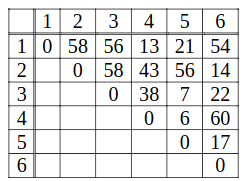
\includegraphics[scale=.8]{19.png}
\end{center}

\underline{Решение:}

\begin{center}
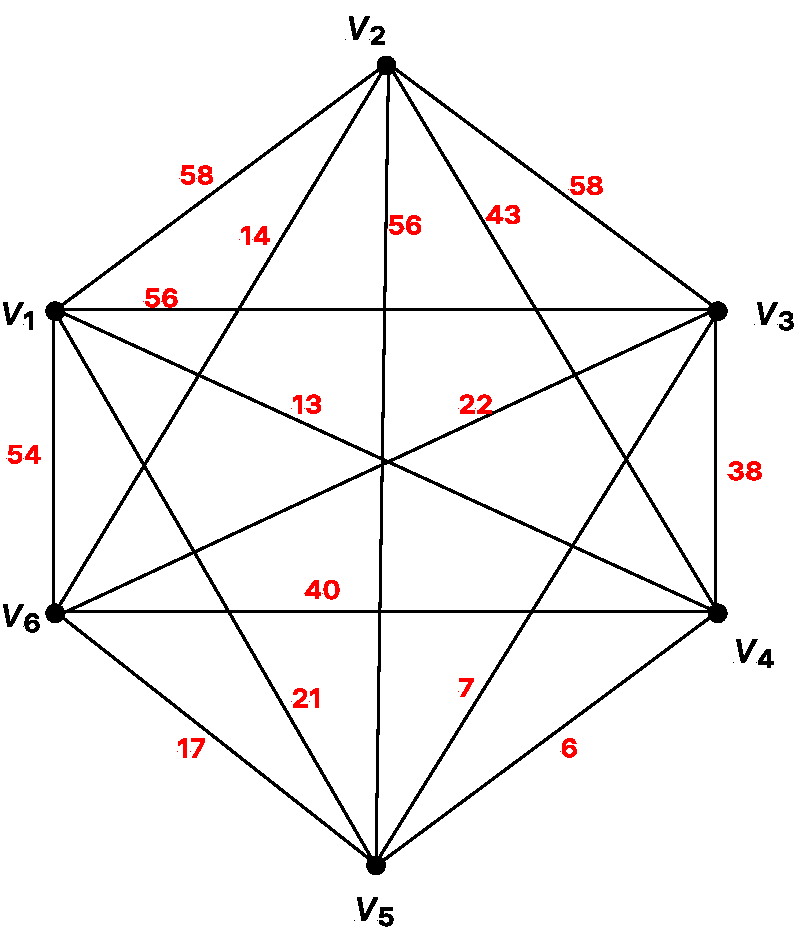
\includegraphics[scale=.6]{19_1.pdf}
\end{center}

Шаг 1. Ребро минимального веса $(v_4, v_5)$ весом 6. Добавляем его. Среди
ребер, инцидентных вершинам $v_4$ и $v_5$  минимальный вес у ребра $(v_5, v_3)$.
Добавляем его. Теперь нужно замкнуть цикл. Добавляем ребро $(v_3, v_4)$.
Получили начальный цикл.

\begin{center}
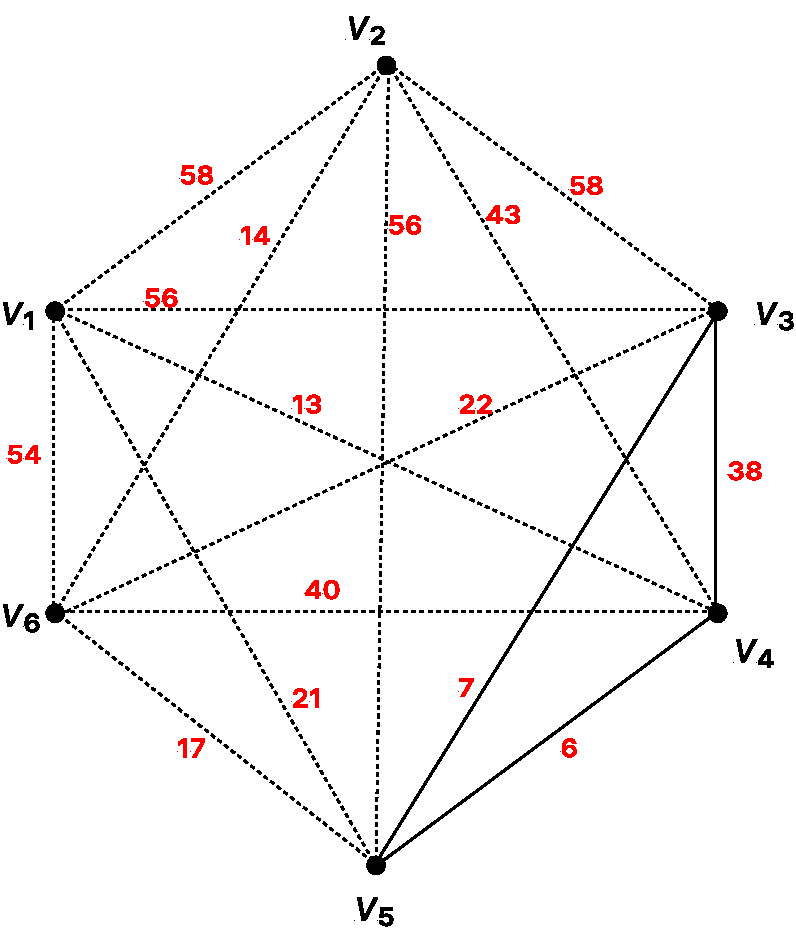
\includegraphics[scale=.6]{19_2.pdf}
\end{center}

Шаг 2. Среди ребер, инцидентных вершинам $v_3$, $v_4$, $v_5$, включенным в цикл,
минимальный вес имеет ребро $(v_4, v_1)$. Добавляем его:

\begin{center}
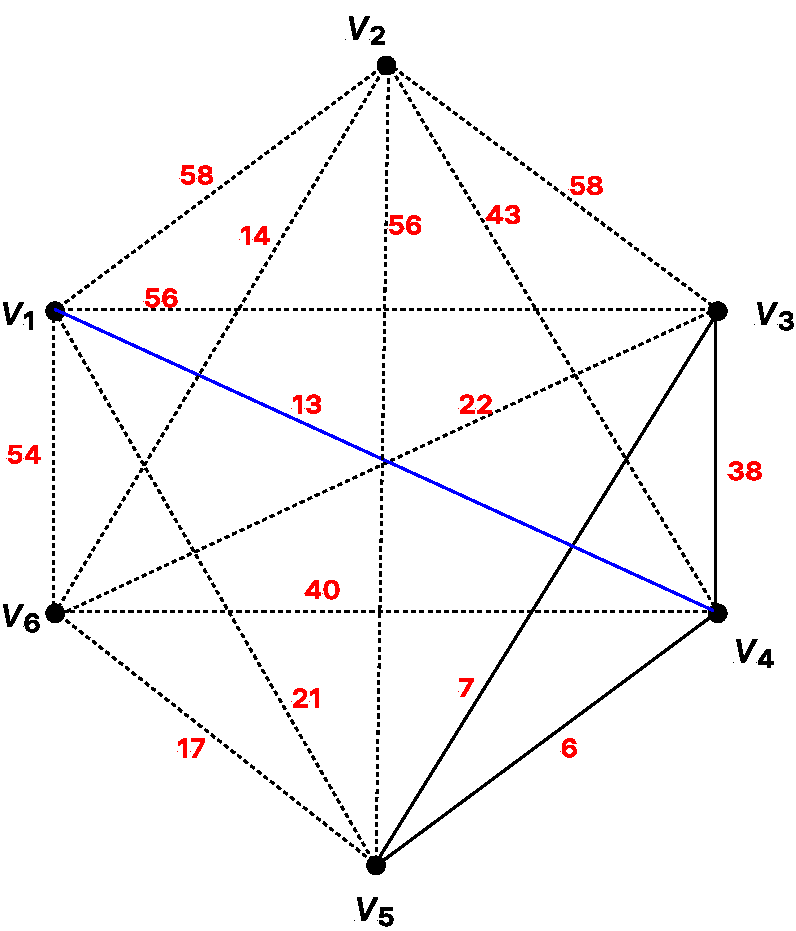
\includegraphics[scale=.6]{19_3.pdf}
\end{center}

У вершины $v_4$ степень 3, значит одно из ребер $(v_4, v_5)$ или $(v_4, v_3)$ нужно исключить. Определим какое:

-$(v_4, v_5)$: -6+21=15

-$(v_4, v_3)$: -38+56=18

Более эффективна первая схема. Получим:

\begin{center}
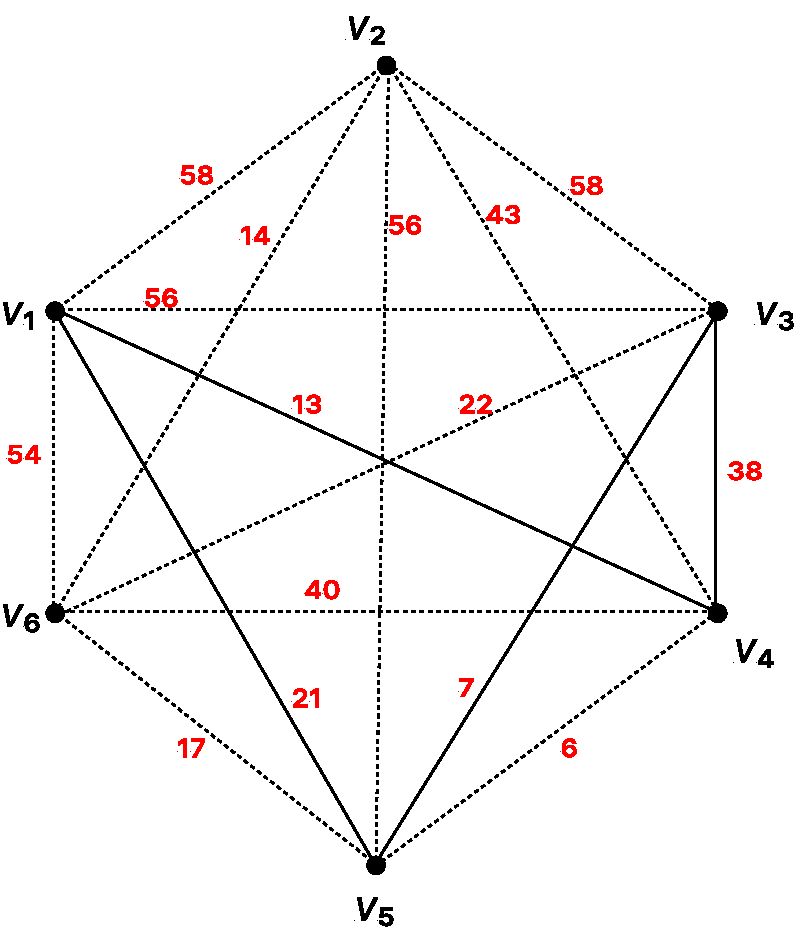
\includegraphics[scale=.6]{19_4.pdf}
\end{center}

Не включена вершина $v_6$. Повторим шаг 2. Минимальный вес у ребра $(v_6, v_5)$
- добавляем его

\begin{center}
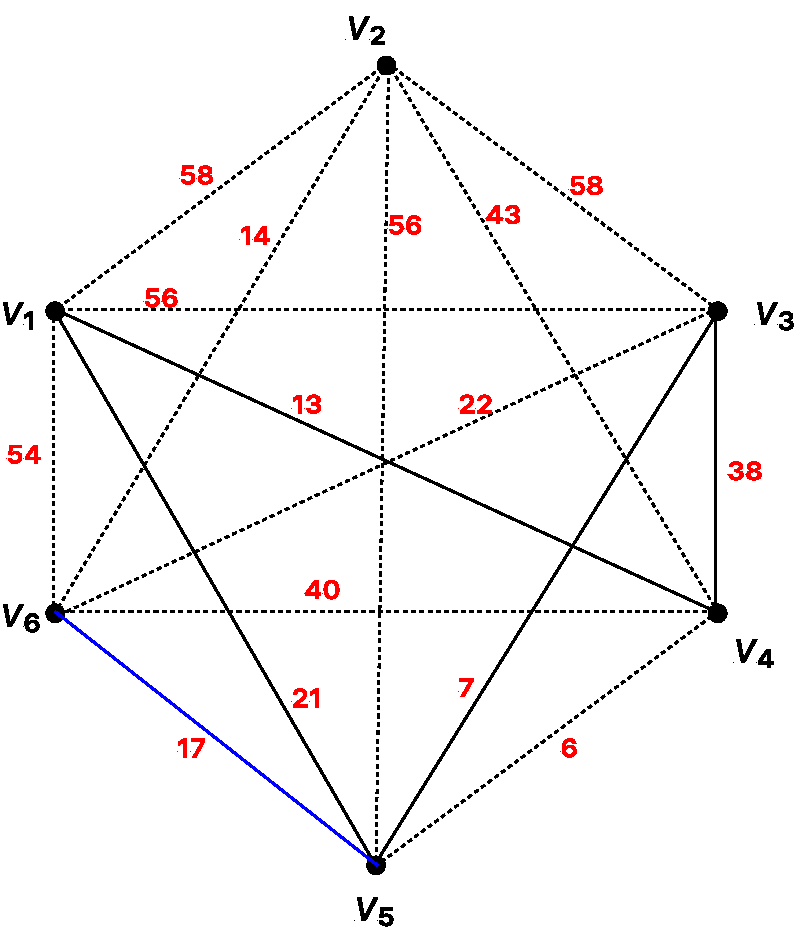
\includegraphics[scale=.6]{19_5.pdf}
\end{center}

Степень вершины $v_5$ стала 3, значит нужно исключить либо $(v_5, v_1)$, либо
$(v_5, v_3)$. Выполним проверку:

-$(v_5, v_1)$: -21+54=33

-$(v_5, v_3)$: -7+22=15

Вторая схема эффективнее. Выберем ее получим:

\begin{center}
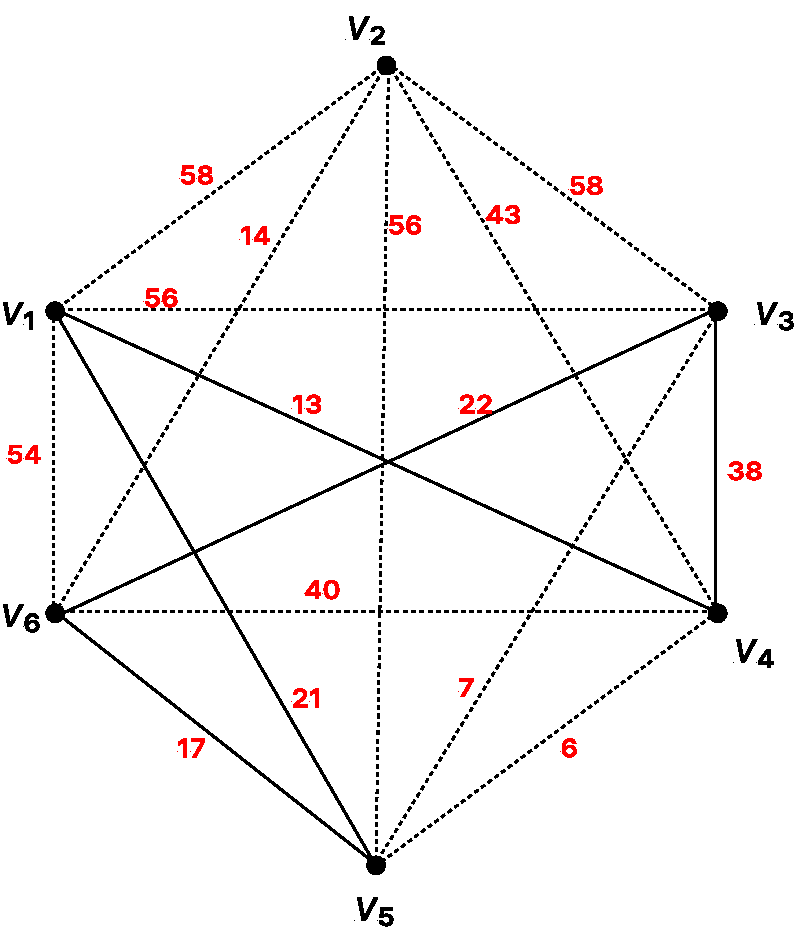
\includegraphics[scale=.6]{19_6.pdf}
\end{center}

Не включена вершина $v_2$. Повторим шаг 2. Минимальный вес у ребра $(v_2, v_6)$ -
 добавляем его.

\begin{center}
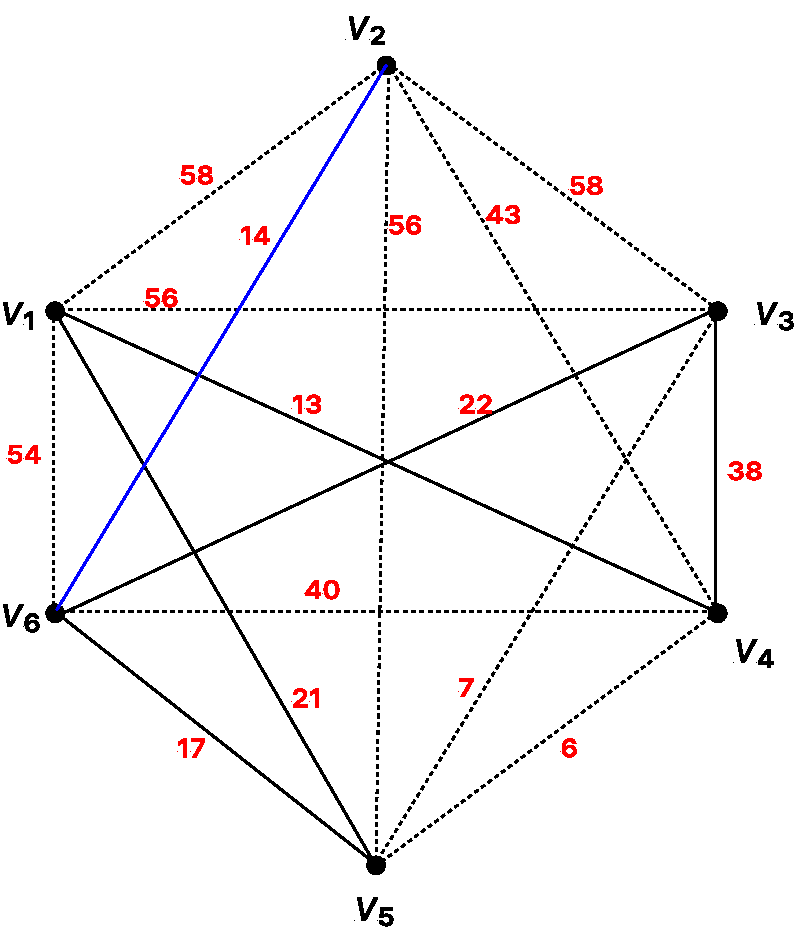
\includegraphics[scale=.6]{19_7.pdf}
\end{center}

Степень вершины $v_6$ стала 3, значит нужно исключить либо
$(v_6, v_3)$, либо $(v_6, v_5)$. Выполним проверку:

-$(v_6, v_3)$: -22+58=36
-$(v_6, v_5)$: -17+56=39

Первая схема эффективнее. Выберем ее получим:

\begin{center}
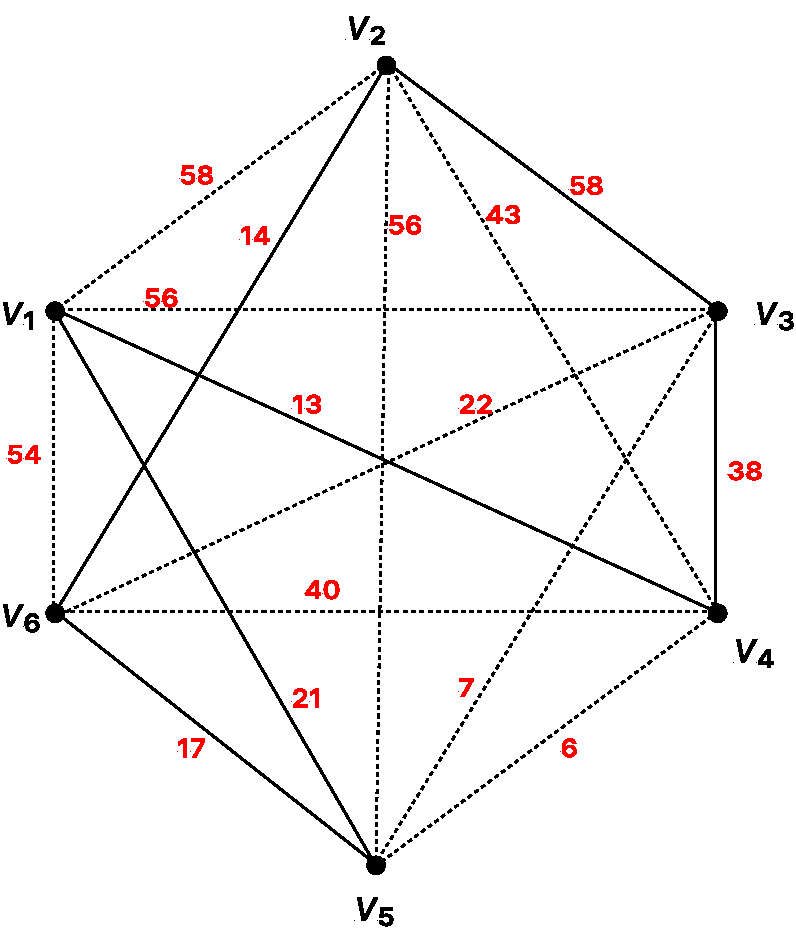
\includegraphics[scale=.6]{19_8.pdf}
\end{center}

Все вершины включены в цикл. Это ответ!

\end{document}
